%-------------------------------------------------------------------------------
% LATEX TEMPLATE ARTIKEL
%-------------------------------------------------------------------------------
% Dit template is voor gebruik door studenten van de de bacheloropleiding 
% Informatica van de Universiteit van Amsterdam.
% Voor informatie over schrijfvaardigheden, zie 
%                               https://practicumav.nl/schrijven/index.html
%
%-------------------------------------------------------------------------------
%	PACKAGES EN DOCUMENT CONFIGURATIE
%-------------------------------------------------------------------------------

\documentclass{uva-inf-article}
\usepackage[english]{babel}
\usepackage{tikz}
\usepackage{pdflscape}
\usepackage{todonotes}

\usepackage[style=authoryear-comp]{biblatex}
\addbibresource{references.bib}

%-------------------------------------------------------------------------------
%	GEGEVENS VOOR IN DE TITEL, HEADER EN FOOTER
%-------------------------------------------------------------------------------

% Geef je artikel een logische titel die de inhoud dekt.
\title{Unreal Engine Live Link Pipeline}

% Vul de naam van de opdracht in zoals gegeven door de docent en het type 
% opdracht, bijvoorbeeld 'technisch rapport' of 'essay'.
% \assignment{}
% \assignmenttype{}

% Vul de volledige namen van alle auteurs in en de corresponderende UvAnetID's.
\authors{Jari Andersen}
% \uvanetids{}

% Vul de naam van je tutor, begeleider (mentor), of docent / vakcoördinator in.
% Vermeld in ieder geval de naam van diegene die het artikel nakijkt!
% \tutor{}
% \mentor{}
% \docent{}

% Vul hier de naam van je tutorgroep, werkgroep, of practicumgroep in.
% \group{SignLab, VisualisationLab}

% Vul de naam van de cursus in en de cursuscode, te vinden op o.a. DataNose.
% \course{}
% \courseid{}

% Dit is de datum die op het document komt te staan. Standaard is dat vandaag.
\date{\today}

%-------------------------------------------------------------------------------
%	VOORPAGINA 
%-------------------------------------------------------------------------------

\begin{document}
\maketitle

%-------------------------------------------------------------------------------
%	INHOUDSOPGAVE EN ABSTRACT
%-------------------------------------------------------------------------------
% Niet toevoegen bij een kort artikel, zeg minder dan 10 pagina's!

%TC:ignore
%\tableofcontents
%\begin{abstract}
%\end{abstract}
%TC:endignore

%-------------------------------------------------------------------------------
%	INHOUD
%-------------------------------------------------------------------------------
% Hanteer bij benadering IMRAD: Introduction, Method, Results, Discussion.
\section{Introduction}
We aim to establish an alternative to the previous pipeline. The previous pipeline incorporated retargeting in Unreal Engine 5 (UE5) and post-processing, among other tasks, in Shogun Post. The alternative pipeline will utilize the functionalities of the Live Link Plugin. With the new pipeline, we will directly stream all data to a Metahuman (or another avatar) in UE5. Similar approaches have been adopted by other projects \cite{auslan, Kara}. While a direct comparison of the two pipelines is unavailable, we can speculate on the advantages and disadvantages of a Live Link Pipeline.

One advantage is the ability to visualize animations directly on an avatar within a scene in UE5. Another is achieving synchronization using the take recorder, eliminating the need to switch between different applications during each recording to verify correctness.

A drawback of this approach is the lack of interaction with marker data during post-processing in Shogun Post. This means issues such as jitters cannot be addressed directly. However, the significance of this drawback is unclear as we aim to capture recordings where such problems are minimized through proper calibration. Another aspect to consider is retargeting animations from one avatar to another. Since the Live Link Pipeline requires retargeting an actor to the avatar being streamed to, we lose the original actor's movements (unless we record in Shogun simultaneously). I have performed target avatar to target avatar retargeting before, and as with all retargets, there was a loss in animation quality. Currently, Shogun Post features an effective auto-retargeter that outperforms manual retargeting in UE5. Therefore, if we intend to switch avatars after recording with the take recorder, we need to consider this aspect. This likely entails applying post-processing in the Animation Sequencer of UE5 to address any discrepancies.

In the remainder of this report, I strive to describe the pipeline. I will skip parts already discussed in the other pipeline, such as Shogun calibration, and parts that require further exploration and practice. A summary of the pipeline can be seen in Figure \ref{fig:pipeline}.

\begin{landscape}
\vspace*{\fill}
\begin{figure}[hbt!]
    \centering
    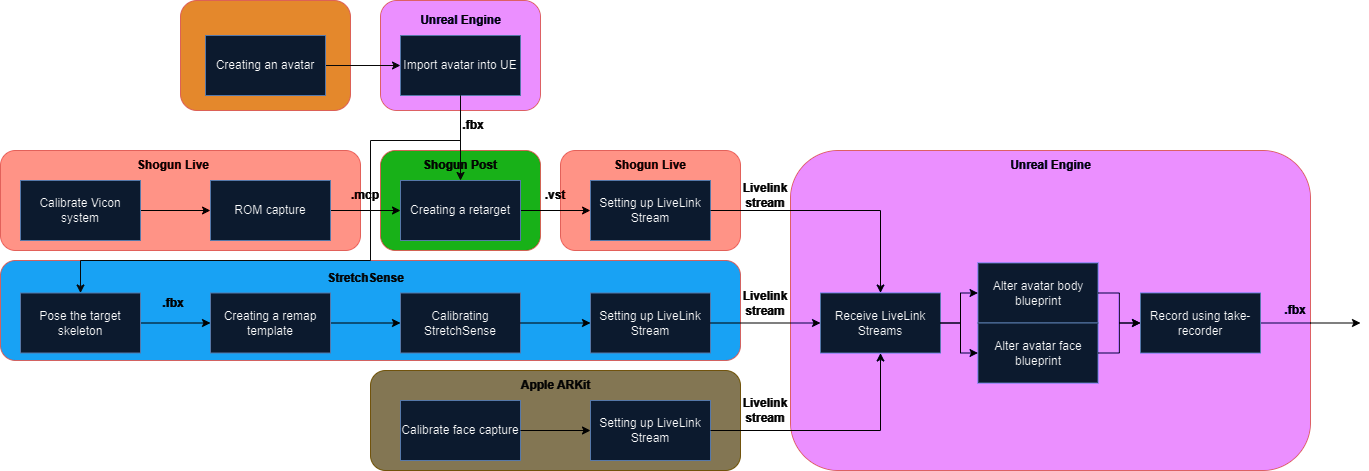
\includegraphics[width=1.5\textheight]{imgs/pipeline16-2-24.png}
    \caption{Current Live Link Pipeline. Three streams into Unreal Engine}
    \label{fig:pipeline}
\end{figure}
\vspace*{\fill}
\end{landscape}



\section{Shogun Live \& Post}
\subsection{Shogun Live ROM}
In the Live Link Pipeline, retargeting is no longer done in UE5 but in Shogun Post. For effective retargeting, Vicon recommends utilizing a "Range Of Motion" (ROM) motion capture. A ROM provides the most accurate rotations and limitations of all joints. This allows us to accurately assess whether all movements are replicated correctly. We record the ROM in Shogun Live, and then import the resulting mcp file into Shogun Post to perform the retargeting.

\subsection{Shogun Post retarget}
Since Shogun Post 1.10, we can utilize an automatic script to retarget a Vicon Skeleton to a Metahuman, including the hands. After importing the ROM mcp and the Metahuman FBX into Shogun Post, we invoke this script by clicking the "TargetMetahuman" button in the "AutoRetargeting" tab or by entering "SetupRetargetToUE5Mannequin;" in the command line. To verify the success of the retargeting, we click the "Retarget over play range" button in the "Subject Setup" tab. If the source and target skeletons match during the animation, the retargeting is successful. However, there is often an issue with incorrect offsets causing the target skeleton to misalign. To resolve this, we align the two skeletons better in "Map Mode". Then, we click "Update Offsets" and upon clicking "Retarget over play range" again, the animation should align properly. We save this retargeting setup as a VSR (Vicon Retarget File) by clicking "Save Retarget Setup".

For other avatars, we have to map mode ourselves from the get go. The ``align skeletons" option in map mode helps us a lot but tweaking is likely needed. Take note that we can only use that option after setting the parts and sides in map mode. After aligning, we auto-create constraints. I have not tested how well this works for the hands, but it seems to perform well for the rest of the body. Similar to the Metahuman retargeting, we validate the retarget gby retargeting over the play range. 

\subsection{Shogun Live Live Link stream}
In Shogun Live, we select the VSR for the "subject" under the "Properties" tab. Now we have completed the setup on Vicon's side. For a video tutorial, please follow Vicon's next video: \url{https://www.youtube.com/watch?v=7LplGd6nKG8}.

\subsection{Known issues}
\begin{itemize}
    \item Due to a bug, the Live Link stream in Unreal Engine may not always work when starting your project in UE. To ensure that we still receive the stream in Live Link, we review a take in Shogun Live where the actor is clearly visible. Afterward, we stop the review, and the stream should start working.
    \item Do not give a name with special characters to an actor in Shogun Live or your takes. Otherwise, the mcp file will no longer work in Shogun Post.
\end{itemize}



\section{StretchSense}
\subsection{Pose Matching}
For StretchSense, Pose Matching is also used. On their website, there is a description of how the avatar's pose should be: \url{https://stretchsense.my.site.com/defaulthelpcenter26Sep/s/article/Fidelity-and-SuperSplay-Glove-Unreal-Engine-Streaming}. However, this cannot be done in the Hand Engine software. It is recommended to use software such as Blender, Cinema 4D, Autodesk, etc. The task here is to pose the avatar in a T-pose and provide the following characteristics:
\begin{enumerate}
    \item Hand palms must point directly downwards and be parallel to the ground.
    \item Fingers must be extended, parallel to each other, and aligned along an axis.
    \item Thumbs must be perpendicular to the other fingers, pointing along an axis.
    \item The thumbnail must point towards the body (not always the case).
\end{enumerate}

Sometimes, even after a perfect Pose, the retarget may still produce undesirable results. This is because the target skeleton is different from the source skeleton (different bone lengths and other proportions). To ensure better results, you can adjust the pose (for example, giving pre-rotations to certain bones).

After a meeting with StretchSense we received extra pointers regarding good thumb retargeting. Instead of pointing the thumbnail towards the body, we can try to rotate it in the range of towards the body and fully upwards.


\subsubsection{Exporting and notes on coordinate systems}
Each of the aforementioned software has its own method of importing and exporting avatars. If the final retarget causes the bones to rotate in the wrong directions, it's often because the export from this step didn't go well. Here is further information on why we encounter this specifically for  \textbf{Unreal Engine's coordinate system}.
One of the notable differences between UE and some other 3D software packages or game engines is their choice of coordinate systems and up axis.
In Unreal Engine, the default coordinate system is the "left-handed coordinate system," where the positive X-axis points to the right, the positive Y-axis points forward, and the positive Z-axis points up. This means that the Z-axis is considered the "up" axis in UE.
In most other 3D software packages or game engines, the default coordinate system is the "right-handed coordinate system," where the positive X-axis points to the right, the positive Y-axis points up, and the positive Z-axis points forward. In this coordinate system, the Y-axis is considered the "up" axis.

Because of this difference in the choice of up axis, when importing assets (such as models, animations, or scenes) from other software packages into Unreal Engine, you may encounter issues related to the orientation or alignment of the objects.

When importing into UE, we can give a pre-rotation to the FBX. This can help orient the avatar correctly before inputting it in in UE.
Regardless, we would prefer the export of a skeleton to be correct.

In Blender, we encountered such a problem when trying to retarget to a ReadyPlayerMe avatar. The export settings that helped us at that time are displayed in figure
\ref{fig:blenderSettings}.
\begin{figure}
    \centering
    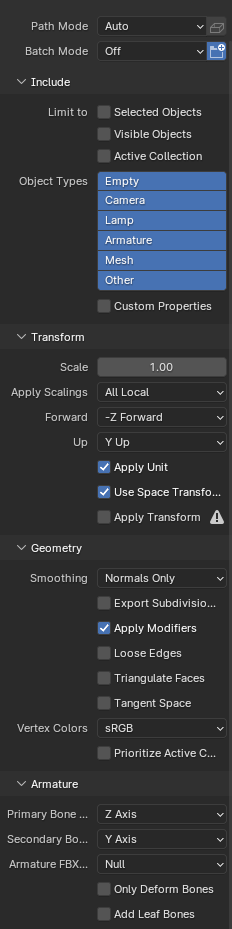
\includegraphics[height=0.9\textheight]{imgs/settings.png}
    \caption{Blender export settings for UE}
    \label{fig:blenderSettings}
\end{figure}

StretchSense has notified us that the coordinate system of Hand Engine is the same as Unreal's coordinate system. In addition, using a good primary bone axis in the export out of Blender is also important. If u see the retarget working in the correct directions, but the mesh of each part are turning in the wrong direction, then you are not using correct bone axis.


\subsection{StretchSense retarget template}
StretchSense will ultimately control the fingers on the target avatar. For this, the skeleton of StretchSense hands needs to be retargeted onto the hands of the avatar. We create this retarget under the \textit{Tools $>$ Remapping} tab. Select the target avatar FBX file to retarget to, and indicate which bones correspond to each other for all "bones". After saving this, we can select the remap for both hands. A supporting image to reference is Figure \ref{fig:sslabels}.

Some tips:
\begin{itemize}
    \item Not all bones need to be retargeted (sometimes leaf bones don't do anything).\\Important to note however, if we don't use the metacarpals we won't be able to mimic cupping motions.
    \item The 1, 2, and 3, hand bones for the HE hands, correspond to the actual finger bones. 0 is for the metacarpal.
    \item Don't forget to set the correct hands. After reusing a template the hands will be reset.
\end{itemize}

\begin{figure}
    \centering
    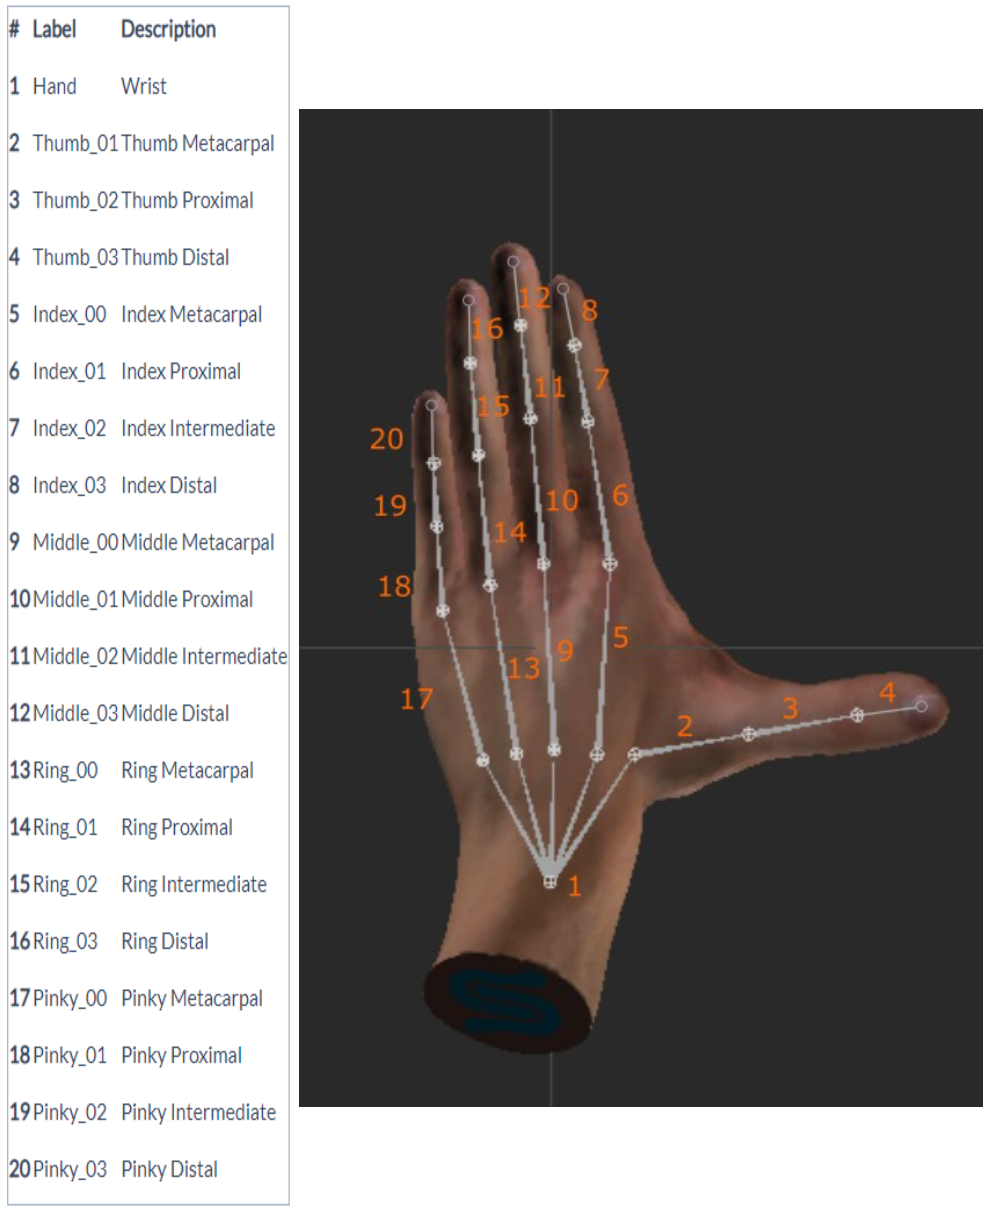
\includegraphics[height=0.6\textheight]{imgs/StretchSenseMapping.png}
    \caption{The bone labeling for the StretchSense hands}
    \label{fig:sslabels}
\end{figure}

\subsection{Calibrating StretchSense}
A lot of testing is still needed to figure out what works best.
\todo{Ask Oline for summary}


\subsection{StretchSense Live Link stream}
Enable "TCP Streaming" for both hands. Under the hands in the UI, we can read the status of the stream.
All information can be found on the StretchSense website: \url{https://stretchsense.com/news/using-stretchsense-gloves-to-power-a-metahuman/}.
This works the same for other avatars.

Bugs HE PRO 3.0.6:
\begin{itemize}
    \item Currently, there is a bug in the remap and live stream. The remap is given to UE when opening the stream. This means that if you want to use a different remap, you need to remove the live link stream and add it again.
    \item When we open HE it crashes immediatly. This can be due to the computer not being connected on the same wifi as shogun is broadcasting on??? \todo{Figure this out}
\end{itemize}


\subsection{StretchSense Timecode}
To synchronize the StretchSense data with Vicon, we do this in the Timecode tab. DON'T forget to enable this every time you reopen Hand Engine.


\section{Live Link Face}
Live Link Face is installed on an iPhone as an application. Therefore, the following steps should be performed on the iPhone.

\subsection{Calibrate and setup Live Link Face}
At the bottom right of the Live Link Face app, there is an option to recalibrate. Keep your face in a neutral pose for the best calibration.

In the "settings menu" at the top left, we can adjust options such as frame rate, head rotation, timecodes, and streaming. If we don't turn off head rotation, both Vicon and Live Link Face will apply head rotation later. Therefore, turn this off here.\\
Under "Streaming," add the IPv4 address of the target computer (in our case, the desktop). Be careful not to have too many targets listed here (preferably only 1 target), otherwise, the iPhone will send data to too many addresses, causing the stream to be very laggy.

Information about the complete process of streaming on a Metahuman with Live Link Face can be found on the EpicGames website: \url{https://dev.epicgames.com/documentation/en-US/metahuman/animating-metahumans-with-livelink-in-unreal-engine}.

Tips:
\begin{itemize}
    \item Recording may be bugged due to full memory. Keep it clean.
    \item Check if the phone is on the same network as the host computer.
    \item Check IP addresses.
\end{itemize}


\section{Unreal Engine}
In Unreal Engine, we will receive and play all Live Link streams on an avatar. Before we can do this, we need to install a few plugins:
\begin{itemize}
    \item Mocap Pro Live Link
    \item Vicon DataStream LiveLink
    \item The following plugins are included by default with UE5 after importing a Metahuman, make sure they are enabled:
    \begin{itemize}
        \item Live Link
        \item Live Link Control Rig
        \item Apple ARKit
        \item Apple ARKit Face Support
    \end{itemize}
\end{itemize}

\subsection{Receiving all Live Link streams in Unreal Engine}
In the ``Window $>$ Virtual Production $>$ Live Link" tab, we can receive all Live Link streams. Only the stream from the iPhone is automatically added. To add Vicon and the StretchSense gloves, you add a "Source" at the top left. If the plugins are installed correctly, Vicon will appear as "Vicon Data Stream Source," and StretchSense will appear as "Mocap Pro Glove." The gloves come in on separate ports, so don't forget to add both.

In addition, for debugging and developing purposes, we can use different views when the data is being streamed to inspect the data (see Figure \ref{fig:livelinkoptions}).

\subsection{Combining StretchSense and Vicon}
Live Link currently supports an "ARKit Face subject" simultaneously with a "Live Link Body subject" in the Metahuman blueprint. However, when we fill in the Vicon system for the "body," the original animation blueprint for the Metahuman is no longer used. StretchSense's instructions for getting the hands working require modifying that blueprint. To get both working simultaneously, we will also add Vicon's stream to the blueprint. Find the blueprint of the body (these will have names related to the chosen Metahuman's proportion, something like "m\_tal\_nrw\_animbp"). The following needs to be adjusted here:
\begin{enumerate}
    \item Add three "Live Link Pose" nodes and connect them together.
    \item The first node should have the Live Link Subject of Vicon.
    \item The next two nodes should have the Live Link Subject of the StretchSense gloves.
    \item Connect the "Input Pose" at the beginning.
    \item Connect the "Output Pose" at the end.
\end{enumerate}
Because the Vicon Live Link stream contains the entire skeleton, it is important to place it first in the blueprint. Otherwise, the StretchSense hands will be overwritten by the Vicon stream, and we won't see the movements of the StretchSense hands anymore. Figure \ref{fig:animbp} depicts the blueprint.

Note that we use the same method for applying both streams for other avatars.

\begin{landscape}
\vspace*{\fill}
\begin{figure}[hbt!]
    \centering
    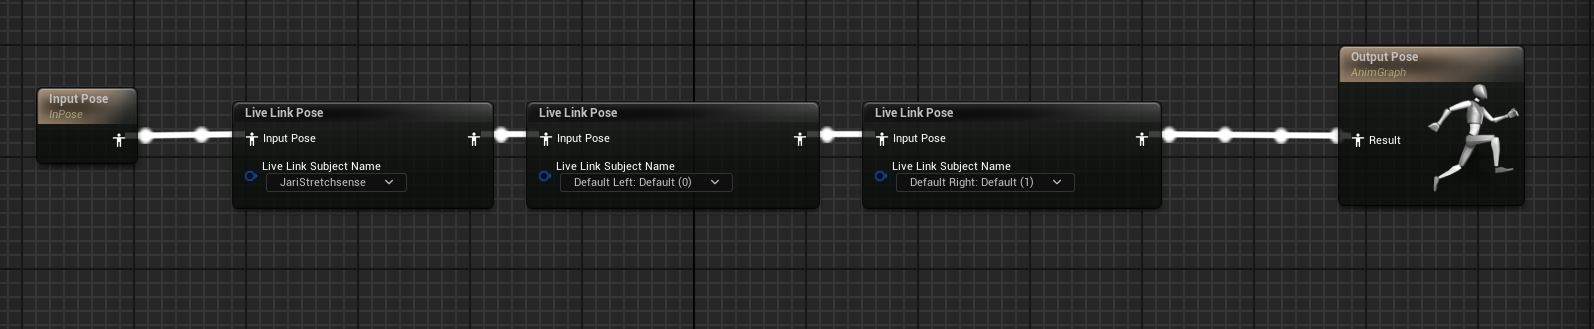
\includegraphics[width=1.5\textheight]{imgs/animbp.png}
    \caption{The modified animation blueprint of the Metahuman. The "Input Pose" is connected to the Live Link Pose (named "JariStretchsense" because the actor has this name in Shogun Live), which is connected to both hands, and the total stream is played on the "Metahuman Output Pose."}
    \label{fig:animbp}
\end{figure}
\vspace*{\fill}
\end{landscape}

\subsection{Gaining control over StretchSense data}
In certain scenarios, using the Live Link data as input is not enough for the output. For example, adding pre-rotations, pre-translations, using a single bone to drive multiple bones, etc. In order to facilitate this, we catch the data in the event graph, and alter it in the anim graph. We show how we do this in Figure \ref{fig:ssPrerot}. And we show how we apply this onto an animation in Figure \ref{animgraphssLLF}. 
\begin{figure}[hbt!]
    \centering
    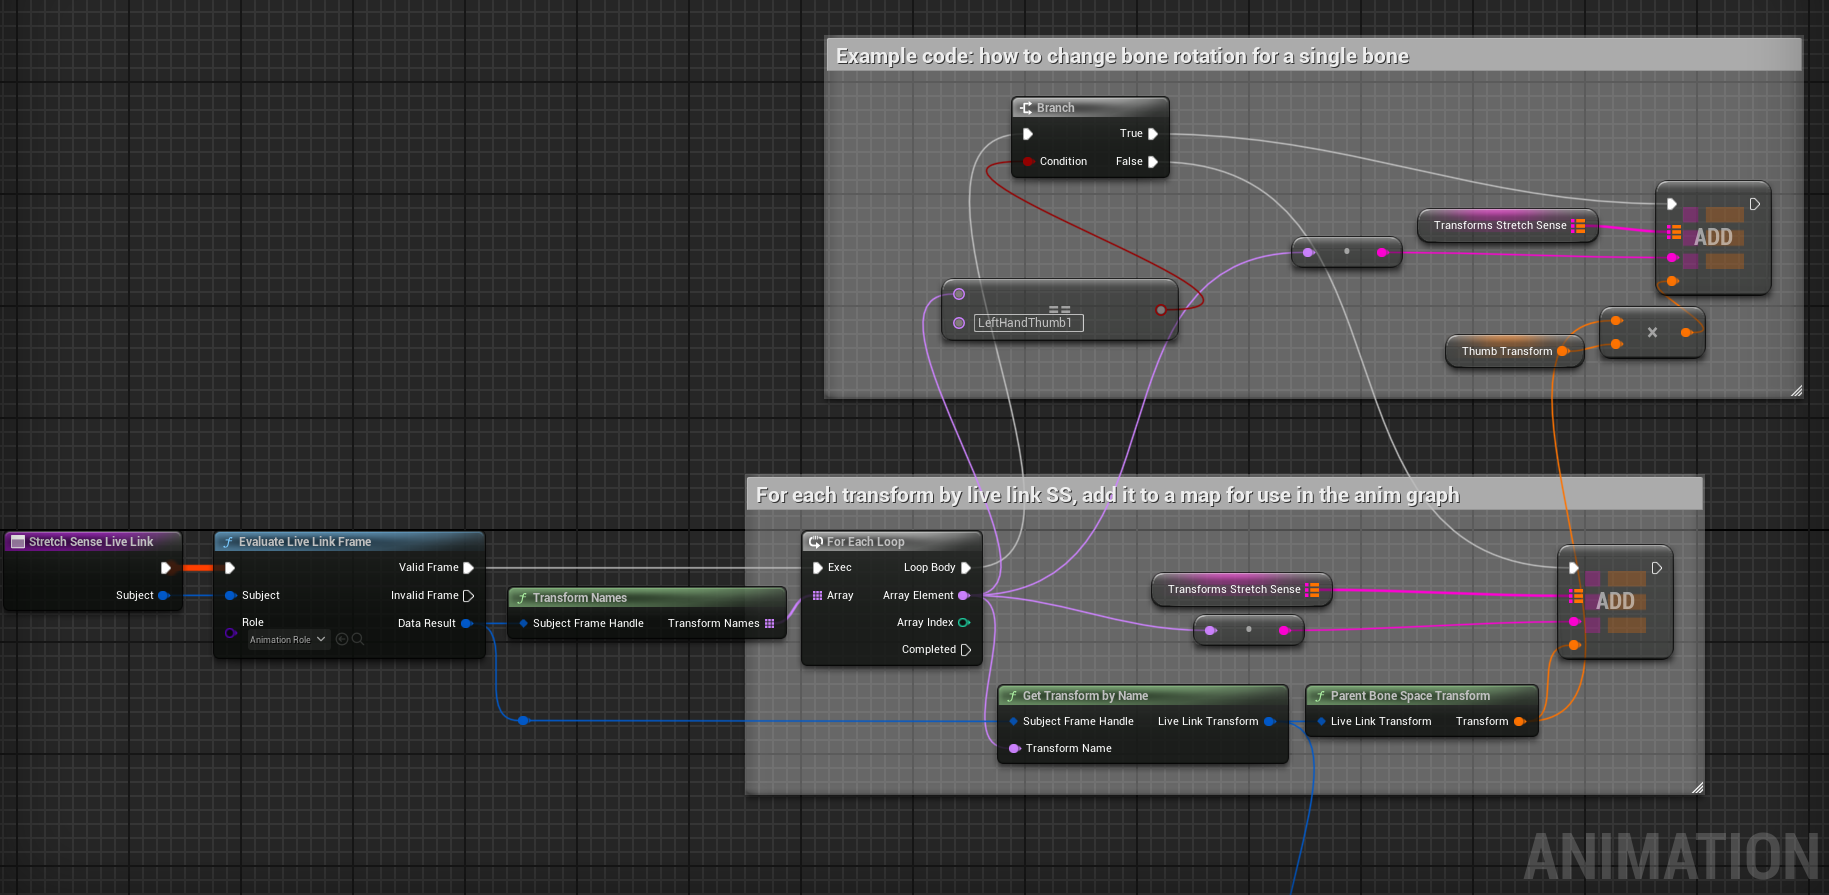
\includegraphics[width=1\textwidth]{imgs/exampleaddingpre-rotation.png}
    \caption{How to catch the StretchSense data and alter it}
    \label{fig:ssPrerot}
\end{figure}



\subsection{Live Link Face on the Metahuman}
In the ``BP\_[Metahuman name]" blueprint of the Metahuman, under ``BP\_[Metahuman name]" in the details tab, there is a Live Link section. Here, you choose the stream from the iPhone for "ARKit Face Subj" and enable the "Use ARKit Face" boolean.

If the head rotation is still being done by this stream, then we need to modify the ``Face\_AnimBP" blueprint. In this blueprint, remove the link between the ``Event Blueprint Update Animation" and "ARKit Head Rotation" nodes.

\subsection{Live Link Face on other avatars}
We can use the Live Link Face application to stream the blendshapes onto other avatars as long as those avatars have blendshapes. 

Tips:
\begin{itemize}
    \item For the ReadyPlayerMe avatars, we append extra information on the download link. If we don't add ``?morphTargets=ARKit", we will not get the ARKit blendshapes.
    \url{https://docs.readyplayer.me/ready-player-me/api-reference/rest-api/avatars/get-3d-avatars}
    \item For the ReadyPlayerMe avatar, the names of the blendshapes are altered. Therefore we could re-write the retarget template blueprint in UE by making a new "retarget asset". This works, but we would prefer a bit more power over the blendshapes. See section \ref{blendshapescontrol} for more information.
\end{itemize}

\subsection{Gaining control over blendshapes}\label{blendshapescontrol}
In our workflow, we rely on the Live Link Face application to transmit blendshapes. While this system serves adequately for some avatars (especially those that share the same blendshape names), it falls short for others. For instance, a smile on a readyplayerme avatar can appear unsettlingly demonic.

To address this, we recognized the need for greater control over the blendshape data we receive. By accessing the "View Options" tab within the Live Link plugin interface (see Figure \ref{fig:livelinkoptions}), we can inspect the incoming data streams.

To exert finer control over this data, we've implemented a C++ and blueprint solution. Initially, we define a remap for the received blendshape data to correspond correctly with our target blendshapes (Figure \ref{fig:datatablesnippet}). This remap structure is defined in C++. Subsequently, we use a blueprint to loop over every value, find the source blendshape value and multiply this by the weight from the datatable. An example of using this weight: reducing the intensity of the smile blendshape by 50\% results in a more natural expression, eliminating the uncanny valley effect.
In addition, this method lets us drive multiple blendshapes with a single blendshape. For example, for the readyplayerme avatar, the lower jaw and teeth have separate blendshapes. By letting the jaw drive the teeth as well, we have a more realistic setup.

To facilitate this process, we store these modified blendshapes in a final map in the event graph (target blendshape to value), which we then apply within the anim graph of the blueprint. This application is achieved using the "Modify Curve" node within the anim graph. The reason why we do this in the anim graph with the modify curve node instead of in the event graph with the "Set morph target" node is because the take recorder doesn't spot the changing values from the event graph.

\begin{figure}[hbt!]
    \centering
    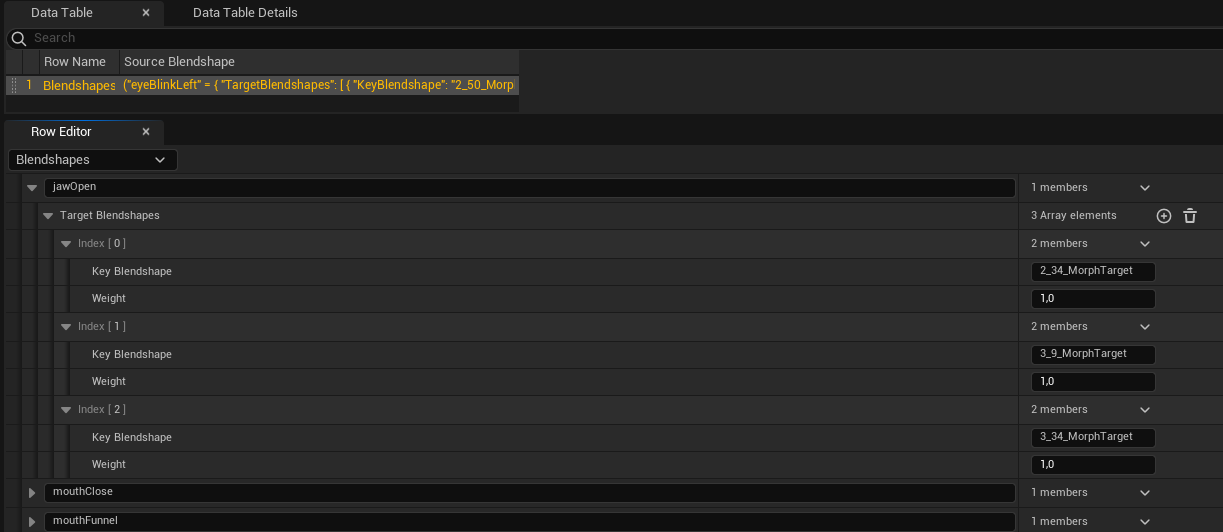
\includegraphics[width=\textwidth]{imgs/blendshapeRemapSnippet.png}
    \caption{A datatable showcasing that a source blendshape is going to drive blendshapes with weights.}
    \label{fig:datatablesnippet}
\end{figure}


\begin{figure}[hbt!]
    \centering
    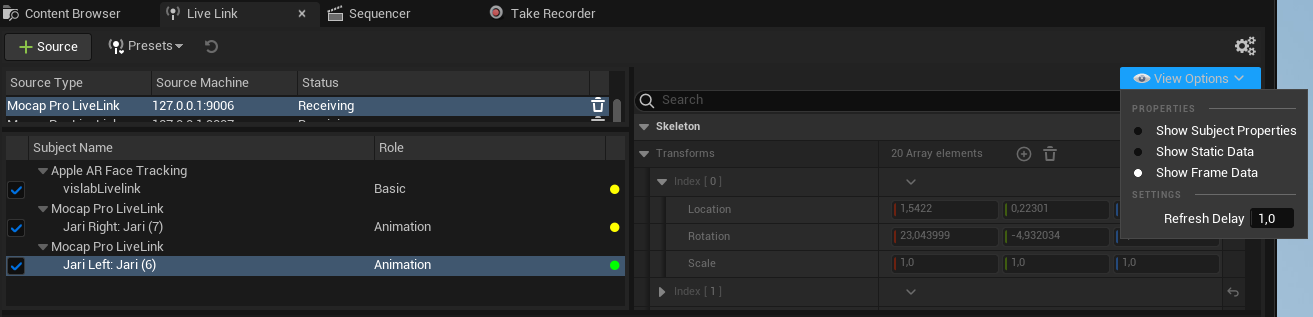
\includegraphics[width=\textwidth]{imgs/livelinkoptions.png}
    \caption{Frame data option for Live Link streams}
    \label{fig:livelinkoptions}
\end{figure}

\begin{figure}[hbt!]
    \centering
    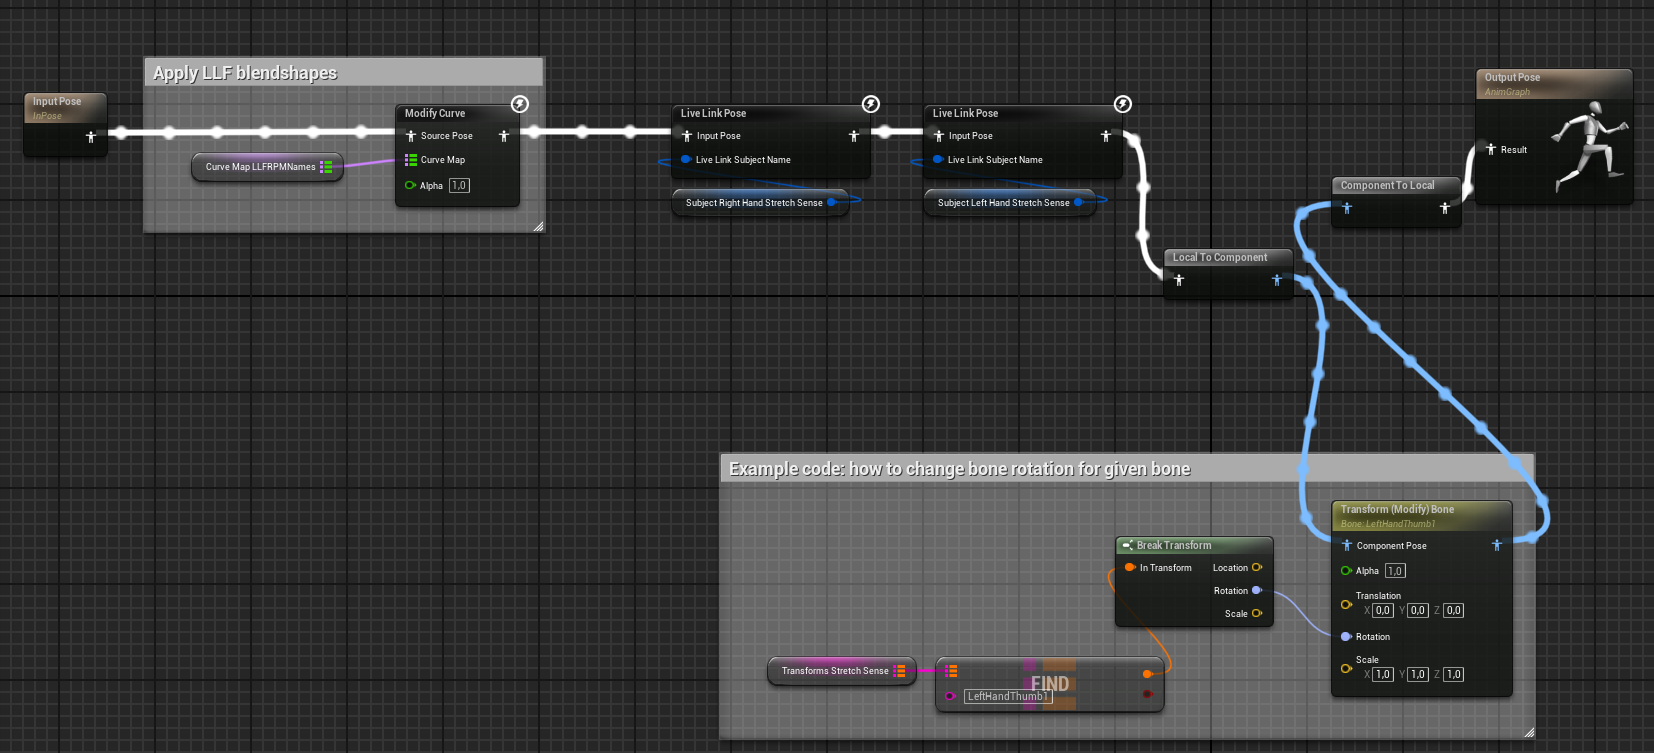
\includegraphics[width=1\textwidth]{imgs/ssAndLLFAnimGraph.png}
    \caption{An Anim Graph, showcasing how we use the created maps to play on an animations.}
    \label{fig:animgraphssLLF}
\end{figure}



\subsection{Recording with the take-recorder}
\todo{Add blueprint/py info and additions we made from the signbank project}

%-------------------------------------------------------------------------------
%	REFERENTIES
%-------------------------------------------------------------------------------

\printbibliography

%-------------------------------------------------------------------------------
%	BIJLAGEN 
%-------------------------------------------------------------------------------

%TC:ignore
% \appendix 
% \section{Bijlage {\LaTeX} code}
% Bijgevoegd zijn de \textattachfile{main.tex}{code} en 
% \textattachfile{references.bib}{bibliografie}.
%TC:endignore

%-------------------------------------------------------------------------------
\end{document}